
\section{McSat: An extension of SMT Solvers}

\subsection{Introduction}


Mcsat is an extension of usual SMT solvers, introduced in~\cite{VMCAI13} and~\cite{FMCAD13}.
In usual SMT Solvers, interaction between the core SAT Solver and the Theory is pretty limited~:
the SAT Solver make boolean decision, and sends them to the theory, whose role is in return to
stop the SAT Solver as soon as the current set of assumptions is incoherent. This means
that the information that theories can give the SAT Solver is pretty limited, and furthermore
it limits the ability of theories to guide the proof search.

While it appears to leave a reasonably simple job to the theory, since it completely
hides the propositional structure of the problem, this simple interaction between the
SAT Solver and the theory makes it harder to combine multiple theories into one. Usual
techniques for combining theories in SMT solvers typically require to keep track of
equality congruence classes and require of theories to propagate any equality they discover.

McSat extends the SAT paradigm by allowing more exchange of information between the theory
and the SAT Solver. This is achieved by allowing the solver to not only decide on the truth value
of atomic propositions, but also to decide assignments for terms that appear in the problem.
For instance, if the SAT Solver assumes a formula $x = 0$,
an arithmetic theory could propagate to the SAT Solver that the formula $x < 1$ must also hold,
instead of waiting for the SAT Solver to guess the truth value of $x < 1$ and then
inform the SAT Solver that the conjunction~: $x = 0 \land \neg x < 1$ is incoherent.

This exchange of information between the SAT Solver and the theories results in
the construction of a model throughout the proof search (which explains the name
Model Constructing SAT).

\subsection{SMT Solver architecture}

We can represent a simplified version of the information flow (not taking into
account backtracking) of usual SMT Solvers, using the graph in fig~\ref{fig:smt_flow}.
In a pure Sat solver, the solver starts by doing
boolean propagation until no more literal can be propagated, at which point it
makes a decision and assign a truth value to a literal not yet assigned. It then
loops to its starting point and does boolean propagation. In an SMT solver,
after each propagation and decision, the solver sends the newly assigned literals
to the theory. The theory then has the possibility to declare the current set of
literals incoherent, and give the solver a tautology in which all literals are currently
assigned to $\bot$, thus prompting the solver to backtrack.

\begin{figure}
  \begin{center}
    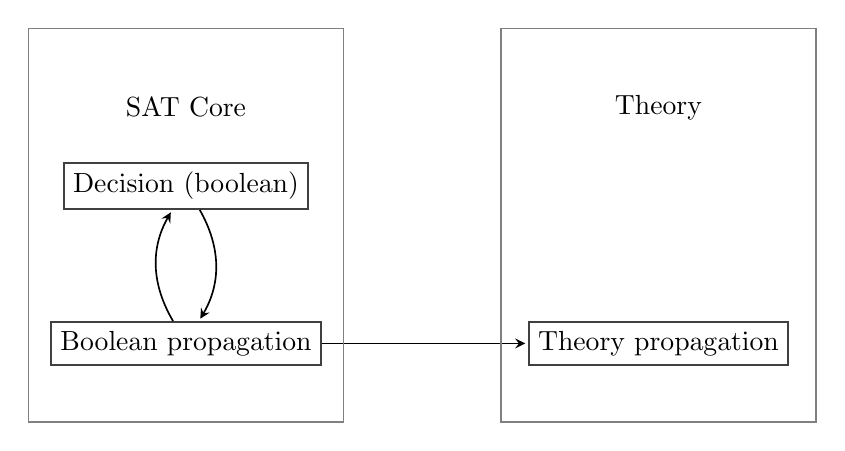
\begin{tikzpicture}[
        ->, % Arrow style
        > = stealth, % arrow head style
        shorten > = 1pt, % don't touch arrow head to node
        node distance = 2cm, % distance between nodes
        semithick, % line style
        auto
      ]

      \tikzstyle{state}=[rectangle,draw=black!75]

      \node (sat) {SAT Core};
      \node (th) [right of=sat, node distance=6cm] {Theory};
      \node[state] (d) [below of=sat, node distance=1cm] {Decision (boolean)};
      \node[state] (bp) [below of=d, node distance=2cm] {Boolean propagation};
      \node[state] (tp) [right of=bp, node distance=6cm] {Theory propagation};

      \draw (d) edge [bend left=30] (bp);
      \draw (bp) edge [bend left=30] (d);
      \draw (bp) edge (tp);

      \draw[black!50] (-2,1) rectangle (2,-4);
      \draw[black!50] (4,1) rectangle (8,-4);

    \end{tikzpicture}
  \end{center}
  \caption{Simplified SMT Solver architecture}\label{fig:smt_flow}
\end{figure}

The main addition of McSat is that when the solver makes a decision, instead of
being restricted to making boolean assignment of formulas, the solver now can
decide to assign a value to a term belonging to one of the literals. In order to do so,
the solver first chooses a term that has not yet been assigned, and then asks
the theory for a possible assignment. Like in usual SMT Solvers, a McSat solver
only exchange information with one theory, but, as we will see, combination
of theories into one becomes easier in this framework.

Using the assignments on terms, the theory can very easily do efficient
propagation of formulas implied by the current assignments.
The information flow then looks like fig~\ref{fig:mcsat_flow}.
For a more detailed presentation, see~\cite{FMCAD13} and~\cite{VMCAI13}.

\begin{figure}
  \begin{center}
    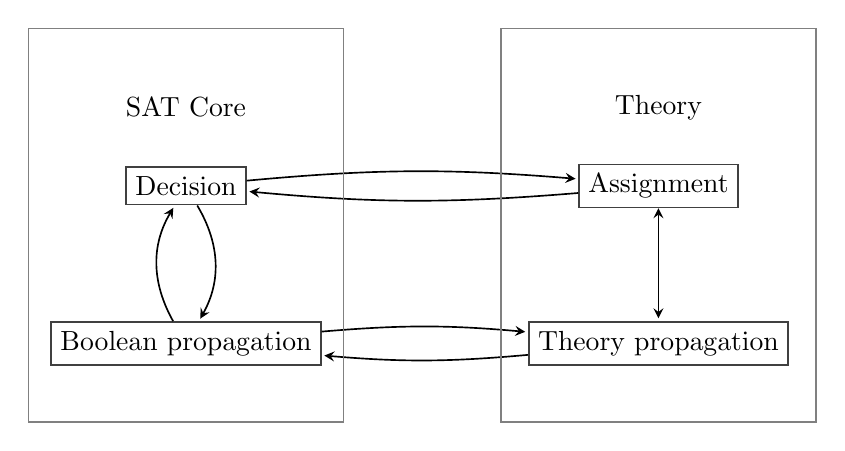
\begin{tikzpicture}[
        ->, % Arrow style
        > = stealth, % arrow head style
        shorten > = 1pt, % don't touch arrow head to node
        node distance = 2cm, % distance between nodes
        semithick, % line style
        auto
      ]

      \tikzstyle{state}=[rectangle,draw=black!75]

      \node (sat) {SAT Core};
      \node (th) [right of=sat, node distance=6cm] {Theory};
      \node[state] (d) [below of=sat, node distance=1cm] {Decision};
      \node[state] (ass) [right of=d, node distance=6cm] {Assignment};
      \node[state] (bp) [below of=d, node distance=2cm] {Boolean propagation};
      \node[state] (tp) [right of=bp, node distance=6cm] {Theory propagation};

      \draw (bp)[right] edge [bend left=5] (tp);
      \draw (tp) edge [bend left=5] (bp);
      \draw (bp) edge [bend left=30] (d);
      \draw (ass) edge [bend left=5] (d);
      \draw (d) edge [bend left=5] (ass);
      \draw (d) edge [bend left=30] (bp);
      \draw[<->] (ass) edge (tp);

      \draw[black!50] (-2,1) rectangle (2,-4);
      \draw[black!50] (4,1) rectangle (8,-4);

    \end{tikzpicture}
  \end{center}
  \caption{Simplified McSat Solver architecture}\label{fig:mcsat_flow}
\end{figure}

\subsection{Decisions and propagations}

In this document, semantic propagations are a bit different from the propagations
used in traditional SMT Solvers. In the case of McSat (or at least the version presented here),
semantic propagations strictly correspond to the evaluation of formulas in the
current assignment. Moreover, in order to be able to correctly handle these semantic
propagations during backtrack, they are assigned a level: each decision is given a level
(typically, it is the number of previous decisions in in the scope when a decision is made),
and a formula is propagated at the maximum level of decision used to evaluate it.

For instance, if the current trail is $\{x \mapsto_1 0, x + y + z = 0 \mapsto_2 \top, y\mapsto_3 0\}$,
then $x + y = 0$ can be propagated at level $3$, but $z = 0$ can not be propagated (at least not
given to the sat solver, however nothing prevents the theory from propagating and using it internally).

\subsection{Models}

Before formalizing the SAT, SMT and McSat algorithms as inference rules, we need to formalize the notion
of partial model. Indeed, during the proof search, the McSat algorithm maintains a partial mapping from
expressions to model values. The intention of this mapping is to represent a partial model of the input
problem, so that if the mapping is complete (i.e all variables are assigned), then it is a model of the
input problem (quantified formula notwithstanding).

More than simply an incomplete model, we also want to be able to give partial function as interpretation of
constants with positive arity. Even further, we'd like to specify these partial interpretations in a somewhat
abstract way, using mappings from expressions to model values instead of a function from model values to model
values. For instance, given a function symbol $f$ of type
$\text{int} \rightarrow \text{int}$ and an integer constant $a$, we'd like to specify that in our mapping,
$f(a) \mapsto 0$, regardless of the values that $f$ takes on other argument, and also regardless
of the value mapped to $a$. To that end we introduce a notion of partial abstract model.

A partial abstract model $\sigma$ is a mapping from ground expressions to model values. To each partial abstract
model correspond a set of models that realize it.

\subsection{Algorithm formalization}

\subsubsection{SAT}

The SAT algorithm can be formalized as follows. During the search, the solver keeps
a set of clauses, containing the problem hypotheses and the learnt clauses, and
a trail, which is the current ordered list of assumptions and/or decisions made by
the solver.

Each element in the trail (decision or propagation) has a level, which is the number of decision
appearing in the trail up to (and including) it. So for instance, propagations made before any
decisions have level $0$, and the first decision has level $1$. Propagations are written
$a \leadsto_C \top$, with $C$ the clause that caused the propagation, and decisions
$a \mapsto_n \top$, with $n$ the level of the decision. Trails are read
chronologically from left to right.

In the following, given a trail $t$ and an atomic formula $a$, we will use the following notation:
$a \in t$ if $a \mapsto_n \top$ or $a \leadsto_C \top$ is in $t$, i.e $a\ in t$ is $a$ is true
in the trail $t$. In this context, the negation $\neg$ is supposed to be involutive (i.e $\neg \neg a = a$),
so that, if $a \in t$ then $\neg \neg a = a \in t$.

The SAT algorithm has two states: first, it starts in the $\text{Solve}$ state, where propagations
and decisions are made, until a conflict is detected, at which point it enters in the $\text{Analyse}$
state, where it analyzes the conflict, backtracks, and re-enter the $\text{Solve}$ state.
The $\text{Solve}$ state take as argument the set of hypotheses and the trail, while
the $\text{Analyze}$ state also take as argument the current conflict clause.

The following invariants are maintained by the transition system:
\begin{description}
  \item[Equivalence] During transitions between states $s_1$ and $s_2$, the set of hypotheses
    (usually written $\mathbb{S}$) in $s_1$ is equivalent to that of $s_2$.
  \item[Trail Soundness] In $\text{Solve}(\mathbb{S}, t)$, if $a \in t$ then $\neg a \notin t$
  \item[Conflict Analysis] In $\text{Analyze}(\mathbb{S}, t, C)$, $C$ is a clause implied by the
    clauses in $\mathbb{S}$, and $\forall a \in C, \neg a \in t$ (i.e $C$ is entailed, yet false
    in the partial model formed by the trail $t$).
\end{description}

\begin{figure}

  Sat Solving
  \begin{center}
    \begin{tabular}{c@{\hspace{1cm}}l}
      % Propagation (boolean)
      \AXC{$\text{Solve}(\mathbb{S}, t)$}
      \UIC{$\text{Sove}(\mathbb{S}, t :: a \leadsto_C \top)$}
      \DP{} &
      $a \in C, C \in \mathbb{S}, \neg a \notin t, \forall b \neq a \in C. \neg b \in t $
      \\ \\
      % Decide (boolean)
      \AXC{$\text{Solve}(\mathbb{S}, t)$}
      \UIC{$\text{Solve}(\mathbb{S}, t :: a \mapsto_n \top)$}
      \DP{} &
      $a \notin t, \neg a \notin t, a \in \mathbb{S}, n = \text{max\_level}(t) + 1$
      \\ \\
      % Conflict (boolean)
      \AXC{$\text{Solve}(\mathbb{S}, t)$}
      \UIC{$\text{Analyze}(\mathbb{S}, t, C)$}
      \DP{} &
      $C \in \mathbb{S}, \forall a \in C. \neg a \in t$
      \\ \\
    \end{tabular}
  \end{center}

  Conflict Analysis
  \begin{center}
    \begin{tabular}{c@{\hspace{1cm}}l}
      % Analyze (propagation)
      \AXC{$\text{Analyze}(\mathbb{S}, t :: a \leadsto_C \top, D)$}
      \UIC{$\text{Analyze}(\mathbb{S}, t, D)$}
      \DP{} &
      $\neg a \notin D$
      \\ \\
      % Analyze (decision)
      \AXC{$\text{Analyze}(\mathbb{S}, t :: a \mapsto_n \top, D)$}
      \UIC{$\text{Analyze}(\mathbb{S}, t, D)$}
      \DP{} &
      $\neg a \notin D$
      \\ \\
      % Resolution
      \AXC{$\text{Analyze}(\mathbb{S}, t :: a \leadsto_C \top, D)$}
      \UIC{$\text{Analyze}(\mathbb{S}, t, (C - \{a\}) \cup (D - \{ \neg a\}))$}
      \DP{} &
      $\neg a \in D$
      \\ \\
      % BackJump
      \AXC{$\text{Analyze}(\mathbb{S}, t :: a \mapsto_d \top :: t', C)$}
      \UIC{$\text{Solve}(\mathbb{S} \cup \{ C \}, t)$}
      \DP{} &
      $\text{is\_uip}(C), d = \text{uip\_level}(C)$
      \\ \\
    \end{tabular}
  \end{center}

  SMT Solving
  \begin{center}
    \begin{tabular}{c@{\hspace{1cm}}l}
      % Conflict (theory)
      \AXC{$\text{Solve}(\mathbb{S}, t)$}
      \UIC{$\text{Analyze}(\mathbb{S}, t, C)$}
      \DP{} &
      $\mathcal{T} \vdash C, \forall a \in C, \neg a \in t$
      \\ \\
    \end{tabular}
  \end{center}

  McSat Solving
  \begin{center}
    \begin{tabular}{c@{\hspace{1cm}}l}
      % Decide (assignment)
      \AXC{$\text{Solve}(\mathbb{S}, t)$}
      \UIC{$\text{Solve}(\mathbb{S}, t :: a \mapsto_n v)$}
      \DP{} &
      $a \notin t, a \in \mathbb{S}, n = \text{max\_level}(t) + 1, \mathcal{T} \vDash t = v \land \bigwedge_{b \mapsto_k v' \in t} b = v'$
      \\ \\
    \end{tabular}
  \end{center}

  \caption{SAT, SMT and McSat inference rules}\label{fig:transitions}
\end{figure}

\subsection{Expected theory invariants}

In the following, we use the following notations:
\begin{itemize}
  \item $\mathbb{V}$ is an infinite set of variables
  \item $\mathbb{C}$ is a possibly infinite set of constants defined
    by a problem's logic\footnote{For instance, the theory of arithmetic
    defines the usual operators $+, -, *, /$ as well as the constants
    $0, -5, \frac{1}{2}, -2.3, \ldots$}
  \item $\mathbb{S}$ is a finite set of constants defined by a problem's type definitions
  \item $\mathbb{T}(\mathbb{X})$ for the (infinite) set of first-order terms over $\mathbb{X}$
    (for instance $a, f(0), x + y, \ldots$)
  \item $\mathbb{F}(\mathbb{T})$ for the (infinite) set of first order quantified formulas
    over the terms in $\mathbb{T}$
\end{itemize}

During proof search are maintained a set of assertions $\mathcal{S}$
and a partial assignment $\sigma$ as a partial function from $\mathbb{T}(\mathbb{V, C, S})$
to $\mathbb{T}(\mathbb{C})$. $\sigma$ is easily extended to a complete substitution function of
$\mathbb{T}(\mathbb{V, C, S})$.

We say that an assignment $\sigma$ is coherent iff $\bigcup_{e\mapsto t \in \sigma} e = t$ is satisfiable
in the current theory (for instance, $\{x\mapsto 1; y \mapsto 2; x + y \mapsto 0\}$ is not coherent).

We say that $\sigma$ is compatible with $\mathcal{S}$ iff for every $\varphi \in \mathcal{S}$,
$\varphi\sigma$ is satisfiable (independently from the rest of the formulas in $\mathcal{S}$).
Intuitively, this represents the fact that the substitution $\sigma$ does not imply any
ground contradictions.

A theory then has to ensure that for every expression $e \in \mathbb{T}(\mathbb{V,C,S})$
there exists $v \in \mathbb{T}(\mathbb{C})$ such that $\sigma' = \sigma \cup \{ e \rightarrow v \}$
is coherent, and compatible with $\mathcal{S}$\footnote{Note that in particular, this implies
that $\sigma$ is coherent with $\mathcal{S}$}. As soon as the current assignment is not coherent,
compatible with the current assertions, or that there is a term $e$ with no viable assignment, the theory
should inform the SAT Solver to backtrack, since the current branch is clearly not satisfiable.
If we reach the point where all expressions of the problem have been assigned, then we
have a ground model for the current set of assertions, which is then also a model
of the input problem.

Of interest if the fact that theories that respect this invariant can easily be combined
to create a theory that also respect this invariant, as long as for any expression $e$,
there is exactly one theory responsible for finding an assignment for $e$\footnote{this
is similar to the usual criterion for combining SMT theories which is that they do not
share symbols other than equality.}.

